\documentclass[12pt,a4paper]{article}
\usepackage{graphicx} % for including images
\usepackage[utf8]{inputenc}
\usepackage{geometry}
\geometry{a4paper, margin=1in}
\usepackage{hyperref} % for hyperlinks
\usepackage{float}
\usepackage{titlesec}

% Define \subsubsubsection
\titleclass{\subsubsubsection}{straight}[\subsection]
\newcounter{subsubsubsection}[subsubsection]
\renewcommand\thesubsubsubsection{\thesubsubsection.\arabic{subsubsubsection}}
\titleformat{\subsubsubsection}
  {\normalfont\normalsize\bfseries}{\thesubsubsubsection}{1em}{}
\titlespacing*{\subsubsubsection}
{0pt}{3.25ex plus 1ex minus .2ex}{1.5ex plus .2ex}

\title{Info2222 Assignment 3 report}
\author{SIDs: 530317166, 510460215}
\date{}

\begin{document}
\maketitle

\section{User Investigation}
\subsubsection*{Persona Overview}
This section presents an analysis of the data collected through a Google Form survey distributed among peers at the University of Sydney. The purpose of the survey was to gather insights to create a detailed persona, which is seen from the table below for our project on enhancing the messaging system used by students.

% Including the persona information as a table
\noindent
\begin{tabular}{|p{0.3\linewidth}|p{0.6\linewidth}|}
\hline
\textbf{Attribute} & \textbf{Details} \\
\hline
\textbf{Photo Name:} & Sam Hong \\
\hline
\textbf{Gender:} & Male \\
\hline
\textbf{Current Role:} & Student \\
\hline
\textbf{Age:} & 20 years old \\
\hline
\textbf{Education/Background:} & Second year University of Sydney Computer Science \\
\hline
\textbf{Area of Interest:} & Cybersecurity, AI, and data science \\
\hline
\textbf{Goal and Tasks:} & To efficiently collaborate on group for academic purposes, and being able to message friends and family \\
\hline
\textbf{Environment:} & Owns a desktop and smart phone, has daily uses for messaging applications \\
\hline
\textbf{Quote:} & \textit{"For academic messaging application, I think, as simple desingn like whatsapp is best"} \\
\hline
\end{tabular}


\subsection*{Methodology}
The survey was shared using an online Google Form, accessible at \url{https://forms.gle/76AmQiAeyXHEHCMZ7}. It aimed to collect diverse opinions and experiences related to the current messaging systems in use by the students.

\subsection*{Demographic and Usage Analysis}
The majority of respondents were male students in their second and third years of study, which provides a clear demographic focus for our user persona. In terms of technology, most respondents reported owning smartphones and desktops, indicating high accessibility to digital platforms. The preferred messaging apps among the participants were Instagram and Discord, which are primarily used for communication between family, friends, and for academic purposes. Furthermore, daily usage of these apps was reported, suggesting a high dependency on digital communication. Regarding navigation preferences, a significant number of users preferred using both mouse and keyboard, which should be considered in designing the interface for enhanced usability.

\subsection*{Feedback Analysis}
\subsubsection*{Features Lacking in Current Systems}
Participants highlighted several features missing from current messaging systems that could enhance their academic experience:
\begin{itemize}
    \item Customization options such as themes, fonts, and layouts to reduce eye strain.
    \item Better organization features like dedicated channels for different subjects or projects.
    \item Enhanced search functions.
    \item Lack of access to marked materials.
    \item Overall sleeker design.
\end{itemize}

\subsubsection*{Challenges Faced}
Respondents identified key challenges with current messaging systems:
\begin{itemize}
    \item Cluttered user interfaces making navigation difficult.
    \item Issues with responsiveness on different devices.
    \item Difficulty tracking important messages in large group chats.
    \item Slow loading times and lack of integration with other academic tools.
\end{itemize}

\subsubsection*{Suggested Improvements}
Based on the limitations identified, the following improvements were suggested:
\begin{itemize}
    \item Options to tag messages or create threads within chats.
    \item Integration of notifications or reminders for academic deadlines.
    \item Faster loading times and simplified user interface.
    \item Easier Log in\&out capabilities
    \item Dedicated section to marked materials
\end{itemize}

\subsection*{PACT Analysis}

\subsubsection*{People}
The users of the system are primarily university students and faculty who interact with the system for communication and content management purposes. The modal functionality directly affects these users, who expect a seamless and intuitive interface for posting and managing content. User expertise may vary significantly, from novice users unfamiliar with web applications to advanced users who are comfortable with digital interfaces.

\subsubsection*{Activities}
 The system is expected to handle daily usage. Users engage in various activities such as sending messages, posting articles, and managing academic content. The system supports real-time communication, content sharing, and collaboration on academic projects. Activities are designed to be straightforward, reducing the cognitive load and enhancing productivity. Users can efficiently manage their academic communications and content through a unified interface. Given its academic uses, there also needs to be management features for staff do control posted content as well as creating marked content that is displayed to the end-user. In tandem, creates a one-stop program to discuss academics and be informed on updated material within said course.

\subsubsection*{Context}
The application is used in an educational environment where reliability and ease of use are crucial. The system is expected to function consistently across various devices and browsers, as users may access the system in different contexts, including during lectures, at home, or while on the move.

\subsubsection*{Technology}
The technology stack includes python, SQl Alchemy and flask for back end server. HTML, CSS, JavaScript (Jinja), and server-side scripting, with elements like modals being crucial for user interaction and dynamic pages. 

\section{Navigation Design }
\subsection*{Card Sorting}

\begin{itemize}
    \item \textbf{Participants:} The session included 3 participants, comprising of target students
    \item \textbf{Materials:} To simulate cardsorting, participants were provided with a Miro link that contains both sticky notes used as categories and rectangle blocks that were used as cards. 
    \item \textbf{Procedure:} Participants were asked to group these cards into categories that seemed logical to them and then label each category.
\end{itemize}

\subsubsection*{Results}
\begin{figure}[H]
\centering
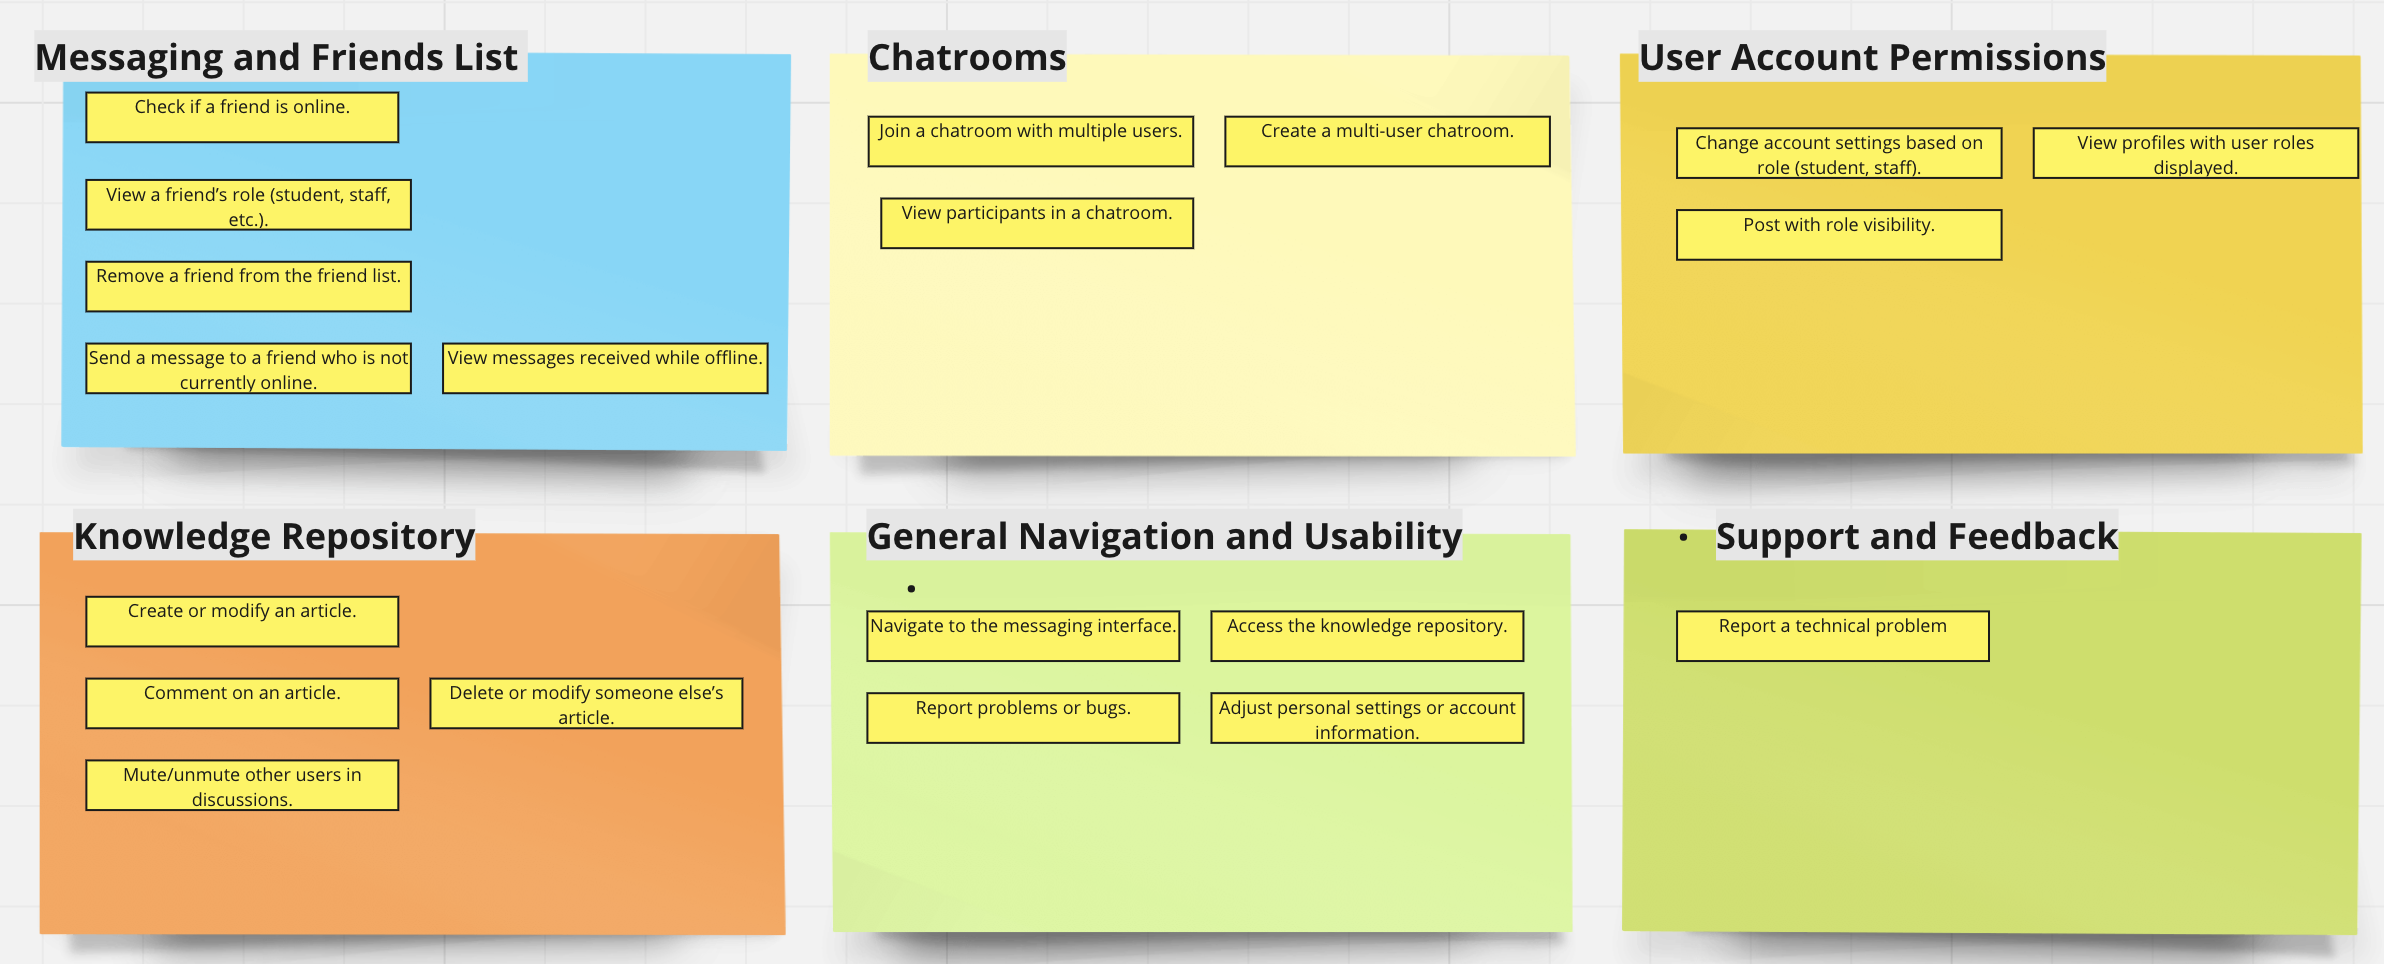
\includegraphics[width=0.8\textwidth]{cardsort.png} 
\caption{Result of cardsort after open and closed card sorting sessions}
\label{fig:sitemap}
\end{figure}


\subsubsection*{Information Architecture}
Based on the results of the card sorting session, the following site map was developed to reflect the user-defined categories and expected navigation paths, again, using Miro.

\begin{figure}[H]
\centering
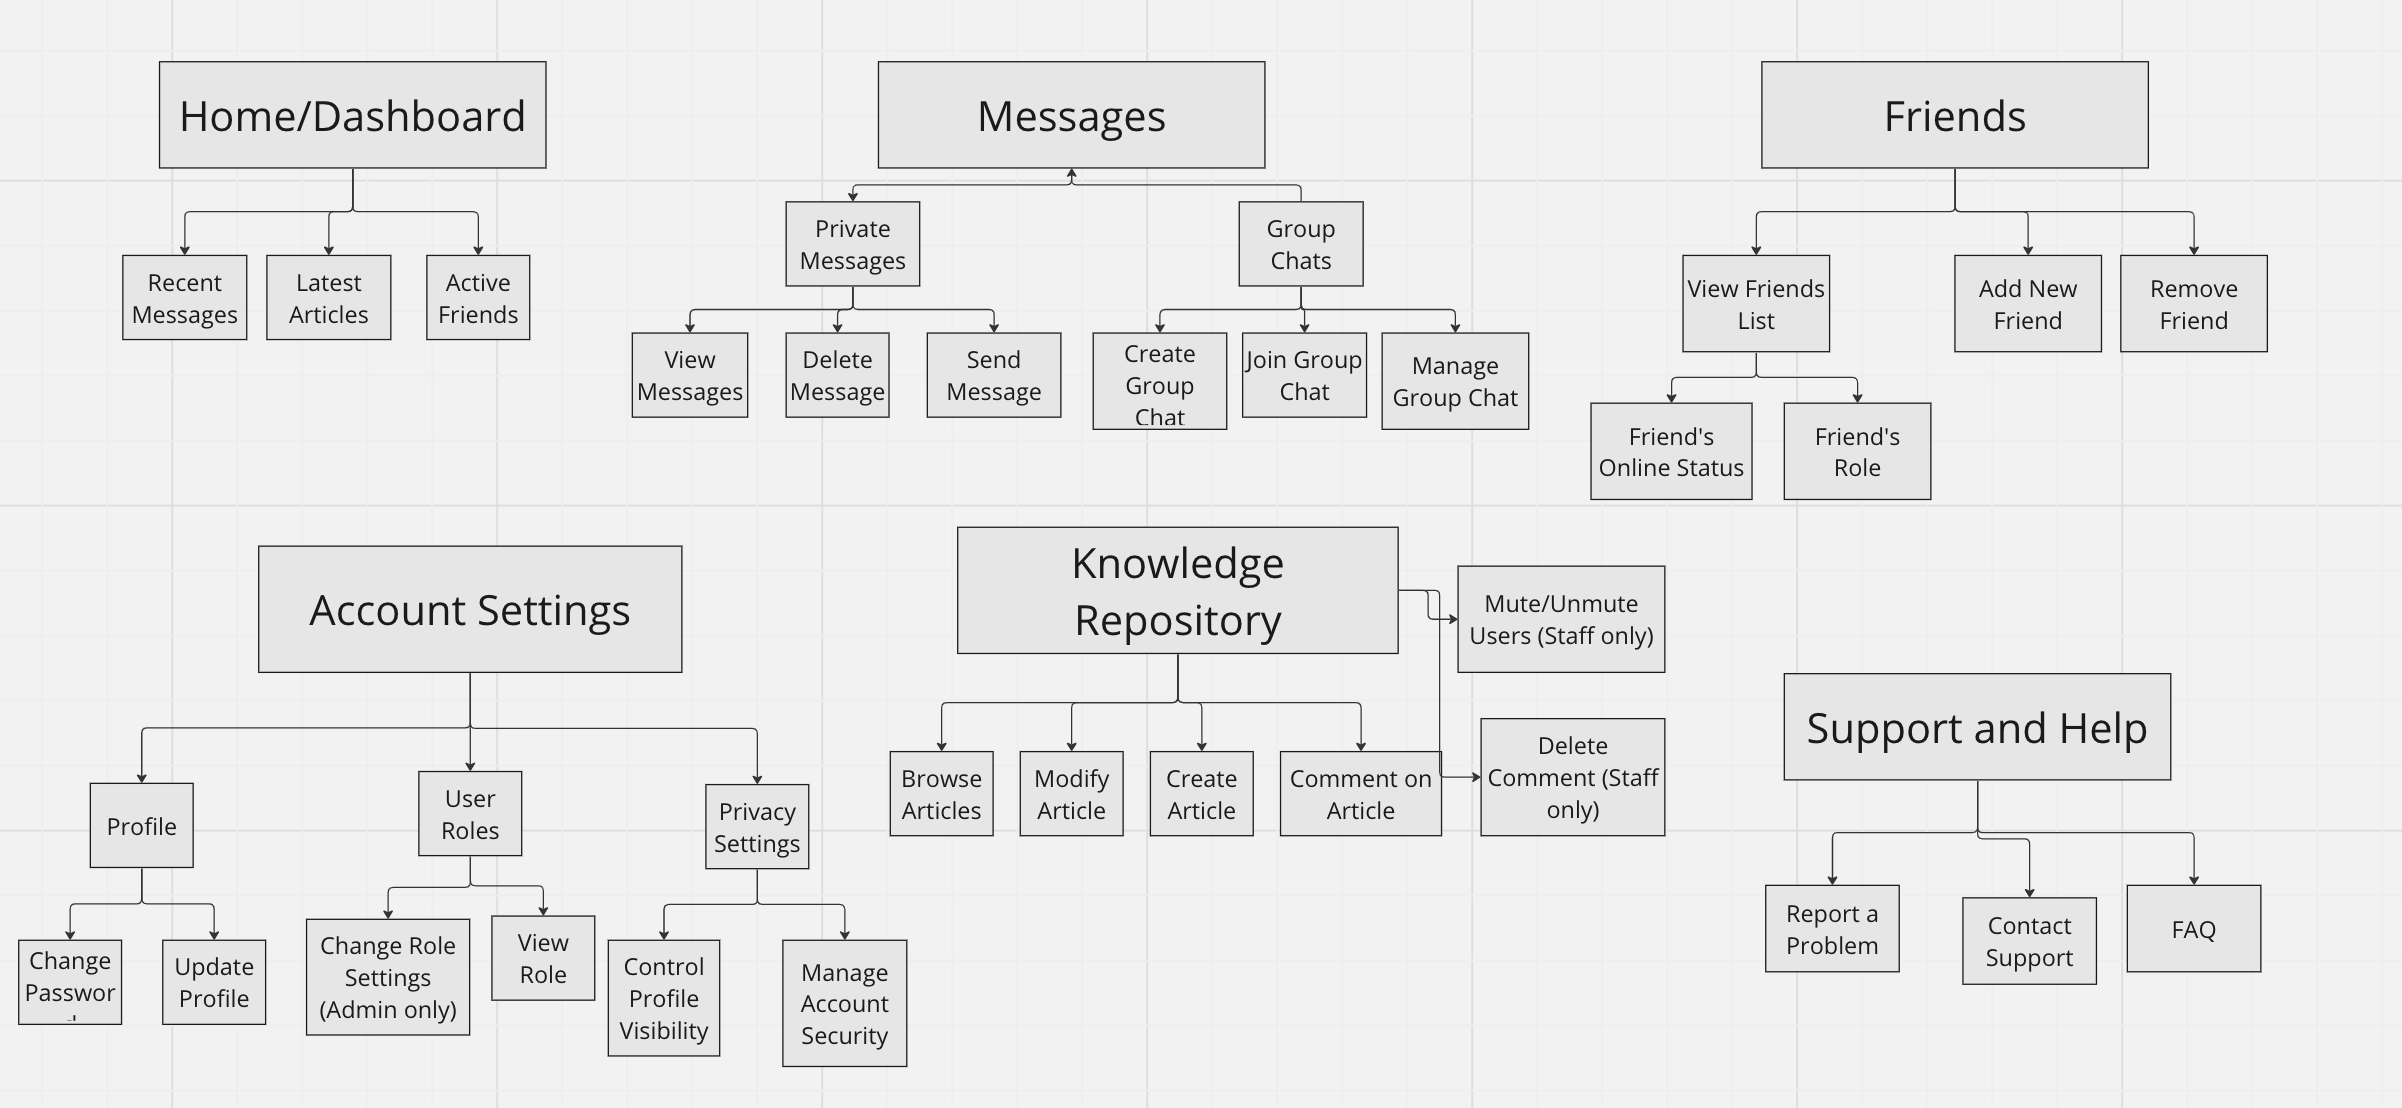
\includegraphics[width=0.8\textwidth]{sitemap.png} % Replace 'sitemap.png' with the actual image file of your site map
\caption{Site Map of the Messaging Platform}
\label{fig:sitemap}
\end{figure}

\section{Design-Evaluate – Low Fidelity or High Fidelity Prototype }
\subsection*{Design Process}
Based on the information architecture derived from the card sorting exercise, we brainstormed and developed initial sketches, which were then translated into digital wireframes. The design focused on simplicity and ease of navigation, aligning with user expectations and feedback.

\subsection*{Prototype Description}
The prototype was developed using miro, featuring the following key sections:

- \textbf{Home Dashboard}: Quick access different chats with friends, quick navigation with articles and posts.

- \textbf{Messages}: Detailed views for private and lobby chats.

- \textbf{Knowledge Repository}: A section for article browsing and interaction.

- \textbf{Assignments}: A section for easily accessible information for assignments.

\begin{figure}[H]
\centering
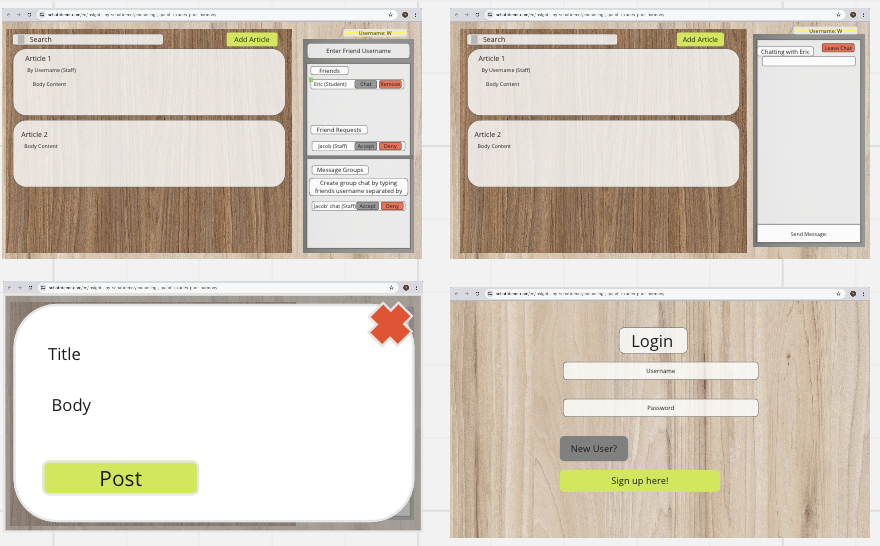
\includegraphics[width=0.8\textwidth]{wireframe.png}
\caption{Wireframe of the Messaging Platform}
\label{fig:wireframe}
\end{figure}

\subsection*{Guerrilla Testing}
\subsubsection*{First Iteration 07/05/24}

\begin{figure}[H]
\centering
\includegraphics[width=0.8\textwidth]{ver1.png} 
\caption{First iteration screen shot}
\label{fig:sitemap}
\end{figure}

\subsubsubsection*{Testing Methodology}
The initial guerrilla testing was conducted among peers from data science courses to gather quick feedback on the early prototype of our application, using a combination of wire frame prototype, basic messaging feature with incomplete core functionalities. 

\subsubsubsection*{Participants}
This iteration involved 2 participants, consisting of both second and first year data sciences students. 

\subsubsubsection*{Findings and Feedback}
The first round of feedback was instrumental in identifying key areas for improvement:
\begin{itemize}
    \item \textbf{Positive Feedback}: Participants appreciated the clear layout and easy navigation of the application, "looks like Omegle".
    \item \textbf{Suggestions for Improvement}:
    \begin{itemize}
        \item Increase the font size to enhance readability.
        \item Profile or username display
        \item Article feature should be fully 
        \item Smoother log out option
    \end{itemize}
\end{itemize}


\subsubsubsection*{Changes Implemented 07/05/24}
Following the feedback from the first iteration, significant changes were made:
\begin{itemize}
    \item The font size was increased across the application to improve text readability.
    \item New, more intuitive icons were introduced for better user experience in navigating the application.
    \item Username included
    \item Log out option
    \item Completed most basic functionalities e.g, articles, lobby chats, log out button. 
\end{itemize}

\subsubsection*{Second Iteration}
\subsubsubsection*{Testing Methodology}
Based on the enhancements made after the first iteration, the second round of guerrilla testing aimed to validate the changes and identify any further improvements needed.

\begin{figure}[H]
\centering
\includegraphics[width=0.8\textwidth]{ver2.png} 
\caption{Second iteration screen shot}
\label{fig:sitemap}
\end{figure}

\subsubsubsection*{Participants}
The same group of participants was involved in the second iteration to assess the changes and provide additional feedback based on the updated version of the application.

\subsubsubsection*{Findings and Feedback}
The second iteration of testing yielded the following insights:
\begin{itemize}
    \item \textbf{Positive Feedback}: Users noted the improvements in readability and navigation, confirming that the changes were effective.
    \item \textbf{Remaining Issues and Suggestions}:
    \begin{itemize}
        \item Some users suggested that the search functionality could be more powerful and faster.
        \item A few participants noted the lack of real-time notifications as a drawback.
    \end{itemize}
\end{itemize}

\subsubsection*{Planned Improvements for the Future}
Following the insights gained from both iterations of guerrilla testing, the following features are planned to be developed and implemented in the future:
\begin{enumerate}
    \item \textbf{Enhanced Search Functionality}: To allow users to quickly find messages and content within the knowledge repository.
    \item \textbf{Real-Time Notifications}: To keep users informed of new messages and updates promptly.
    \item \textbf{Accessibility Improvements}: To ensure the platform is usable by everyone, including users with disabilities.
\end{enumerate}

\subsection{Lighthouse report for Second Iteration}
We conducted an accessibility audit using Google Chrome's Lighthouse tool to ensure that the application is accessible to all users, including those with disabilities. The audit resulted in an overall score of 81 out of 100, indicating a solid foundation but also highlighting areas needing improvement.

\subsubsection{Contrast Adjustment}
The audit identified issues with insufficient contrast ratios between text and background colors, which could impede users with visual impairments. 

\textbf{Actions Taken:}
\begin{itemize}
    \item I reviewed the color schemes used throughout the application and adjusted them to meet or exceed the WCAG 2.1 AA contrast ratio thresholds.
\end{itemize}

\subsubsection{Language Localization}
The absence of a \texttt{[lang]} attribute in the \texttt{<html>} element was noted, which could potentially affect how content is interpreted by screen readers and other assistive technologies.

\textbf{Actions Taken:}
\begin{itemize}
    \item Consider in future adding the appropriate \texttt{lang} attribute to the \texttt{<html>} element to specify the primary language of the document.
\end{itemize}


\subsubsection{Achievements in Accessibility Since Iteration 1}

\begin{itemize}
    \item Ensuring that all interactive elements are accessible via keyboard and have meaningful names.
    \item Maintaining a logical order of headings and labels throughout the application.
    \item Ensuring all forms and controls are labeled correctly, which guarantees their functionality with screen readers.
\end{itemize}


\section{Design-Evaluate (Initial Implementation of Prototype}

\subsection*{Development Approach and Plan}
We utilized GitHub to track changes to our codebase, which can be reviewed at \href{https://github.com/OiBigEarz/info2222-asst2}{our project repository}. https://github.com/OiBigEarz/info2222-asst2. 

\textbf{Iteration Plan:}
\begin{itemize}
    \item \textbf{Iteration \#1 (Weeks 9-10):} Initially, we focused on the basic functionalities, including messaging capabilities, friend management, and laying the groundwork for the UI/UX for future articles. User testing after this iteration provided positive feedback regarding the simplicity of the layout but also pointed out the absence of several expected features such as display of the current username and more intuitive navigation aids.
    \item \textbf{Iteration \#2 (Weeks 11-12):} In response to feedback, the second iteration prioritized the implementation of core functionalities like article management and enhancements in account type functionalities. This phase aimed to refine the user experience and integrate essential features highlighted during the initial user feedback.
\end{itemize}

\subsection*{Contribution Summary}
\subsubsection*{530317166}
Student 530317166 did the following
\begin{itemize}
    \item Report documentation
    \item Card sorting with peers
    \item Conducted Both guerilla testings
    \item Information Architecture site map
    \item User investigation – PACT analysis, Survey
    \item Drawing up prototype/wireframe
    \item UI/UX design for all pages
    \item Account type at sign up
    \item Account permission 
    \item Friend delete
    \item Basic friend features and display
    \item Message storage 
    \item Friend receive message offline
    \item Dynamic messaging chat and room id management
    \item Everything about articles e.g design, post, delete post, edit, comment, delete comment, 
    \item Lobby chat UI
\end{itemize}

\subsubsection*{510460215}
Student 510460215 did the following
\begin{itemize}
    \item User status e.g online/offline
    \item User account type display on friend list
    \item Log out
    \item Player listing for muting 
    \item Lobby chat 
    \item Assignment Section
    \item UI/UX design for pages
\end{itemize}

\end{document}
